\documentclass[openany,preprint,11pt]{article}

\usepackage{amsthm,amsmath,amssymb,amsfonts,amscd,amsbsy}
\usepackage[ruled,noline,linesnumbered]{algorithm2e}
\usepackage{cancel}
\usepackage{color}
\usepackage{fullpage}
\usepackage{graphicx}
\usepackage{hyperref}
\usepackage[tight]{subfigure}
\usepackage{titlesec}

\DeclareGraphicsExtensions{.jpg,.png,.pdf}
\DeclareGraphicsRule{*}{mps}{*}{}
\graphicspath{{./fig/}}



% bold letters
\newcommand{\bola}{\mathbf{a}}
\newcommand{\bolc}{\mathbf{c}}
\newcommand{\bolf}{\mathbf{f}}
\newcommand{\bolg}{\mathbf{g}}
\newcommand{\boll}{\mathbf{l}}
\newcommand{\bolq}{\mathbf{q}}
\newcommand{\bolp}{\mathbf{p}}
\newcommand{\bolu}{\mathbf{u}}
\newcommand{\bolv}{\mathbf{v}}
\newcommand{\bolw}{\mathbf{w}}
\newcommand{\bolz}{\mathbf{z}}

\newcommand{\bolA}{\mathbf{A}}
\newcommand{\bolB}{\mathbf{B}}
\newcommand{\bolC}{\mathbf{C}}
\newcommand{\bolD}{\mathbf{D}}
\newcommand{\bolE}{\mathbf{E}}
\newcommand{\bolF}{\mathbf{F}}
\newcommand{\bolG}{\mathbf{G}}
\newcommand{\bolH}{\mathbf{H}}
\newcommand{\bolI}{\mathbf{I}}
\newcommand{\bolJ}{\mathbf{J}}
\newcommand{\bolK}{\mathbf{K}}
\newcommand{\bolL}{\mathbf{L}}
\newcommand{\bolM}{\mathbf{M}}
\newcommand{\bolN}{\mathbf{N}}
\newcommand{\bolO}{\mathbf{O}}
\newcommand{\bolP}{\mathbf{P}}
\newcommand{\bolQ}{\mathbf{Q}}
\newcommand{\bolR}{\mathbf{R}}
\newcommand{\bolS}{\mathbf{S}}
\newcommand{\bolT}{\mathbf{T}}
\newcommand{\bolU}{\mathbf{U}}
\newcommand{\bolV}{\mathbf{V}}
\newcommand{\bolW}{\mathbf{W}}
\newcommand{\bolX}{\mathbf{X}}
\newcommand{\bolY}{\mathbf{Y}}
\newcommand{\bolZ}{\mathbf{Z}}

% bold symbols
\newcommand{\bolalpha}{\boldsymbol{\alpha}}
\newcommand{\bolbeta}{\boldsymbol{\beta}}
\newcommand{\boleta}{\boldsymbol{\eta}}
\newcommand{\bolpsi}{\boldsymbol{\psi}}

% shadowed letters
\newcommand{\PP}{\mathbb{P}}
\newcommand{\RR}{\mathbb{R}}
\newcommand{\CC}{\mathbb{C}}
\newcommand{\ZZ}{\mathbb{Z}}

% mathcal letters
\newcommand{\calA}{\mathcal{A}}
\newcommand{\calB}{\mathcal{B}}
\newcommand{\calC}{\mathcal{C}}
\newcommand{\calD}{\mathcal{D}}
\newcommand{\calE}{\mathcal{E}}
\newcommand{\calF}{\mathcal{F}}
\newcommand{\calG}{\mathcal{G}}
\newcommand{\calH}{\mathcal{H}}
\newcommand{\calI}{\mathcal{I}}
\newcommand{\calJ}{\mathcal{J}}
\newcommand{\calK}{\mathcal{K}}
\newcommand{\calL}{\mathcal{L}}
\newcommand{\calM}{\mathcal{M}}
\newcommand{\calN}{\mathcal{N}}
\newcommand{\calO}{\mathcal{O}}
\newcommand{\calP}{\mathcal{P}}
\newcommand{\calQ}{\mathcal{Q}}
\newcommand{\calR}{\mathcal{R}}
\newcommand{\calS}{\mathcal{S}}
\newcommand{\calT}{\mathcal{T}}
\newcommand{\calU}{\mathcal{U}}
\newcommand{\calV}{\mathcal{V}}
\newcommand{\calW}{\mathcal{W}}
\newcommand{\calX}{\mathcal{X}}
\newcommand{\calY}{\mathcal{Y}}
\newcommand{\calZ}{\mathcal{Z}}


% derivatives
\newcommand{\pp}[2]{\frac{\partial #1}{\partial #2}}
\newcommand{\dd}[2]{\frac{d #1}{d #2}}


% fraction shortcut
\newcommand{\f}[2]{\frac{#1}{#2}}
\newcommand{\slfrac}[2]{\left.#1\middle/#2\right.}

% common operators
\newcommand{\vvvert}{|\kern-1pt|\kern-1pt|}
\newcommand{\enorm}[1]{\vvvert #1 \vvvert}


% matrices
\newcommand{\bmat}[1]{\left(\begin{array}{#1}}
\newcommand{\emat}{\end{array}\right)} 



\newcommand{\blist}{\begin{list}{\ballrefb}{\leftmargin=2.0em}
  \setlength{\itemsep}{2pt}
  \setlength{\parskip}{0pt}}
\newcommand{\elist}{\end{list}}



% common format strings
\def\etal{{\it et al.}}
\def\ie{{\it i.e.}}
\def\eg{{\it e.g.}}


\DeclareMathOperator*{\arginf}{arg\,inf}
\DeclareMathOperator*{\argsup}{arg\,sup}
\DeclareMathOperator*{\argmax}{arg\,max}
\DeclareMathOperator*{\argmin}{arg\,min}


\newcommand{\disclaimer}{\copyright2018 Masayuki Yano.  Prepared for AER1418 Variational Methods for PDEs taught at the University of Toronto.}

%\titleformat{\chapter}[display]
%            {\huge\bfseries}{Lecture \thechapter}{0.5ex}
%            {} % before code
%            {\disclaimer} % after code
  
%\theoremstyle{definition}
%\newtheorem{theorem}{Theorem}[chapter]
%\newtheorem{lemma}[theorem]{Lemma}
%\newtheorem{proposition}[theorem]{Proposition}
%\newtheorem{remark}[theorem]{Remark}
%\newtheorem{definition}[theorem]{Definition}
%\newtheorem{corollary}[theorem]{Corollary}
%\newtheorem{assumption}[theorem]{Assumption}
%\newtheorem{example}[theorem]{Example}

%\title{Reference manual for FEM2d}
%\author{Masayuki Yano}

\begin{document}
\begin{center}
  \begin{LARGE}
    \textbf{Reference manual for fem2d}
  \end{LARGE}
\end{center}

\noindent\disclaimer
\section{Introduction}
FEM2d is a simple \textsc{Matlab} finite element solver.  The code consists of three functional blocks:
\begin{itemize}
\item \texttt{/mesh}: comprises functions that provide the geometric description of the problem. 
\item \texttt{/ref}: comprises functions that define the reference finite element.
\item \texttt{/driver}: comprises problem-specific driver scripts.
\end{itemize}
In addition, the code contains \texttt{/distmesh} which provides meshing capabilities.  To add all the required directory to the path, call \texttt{setup} in the root directory.


\section{The \texttt{mesh} structure}
We will describe the mesh structure using the following $p=1$ mesh as an example.
\begin{figure}[!h]
  \centering
  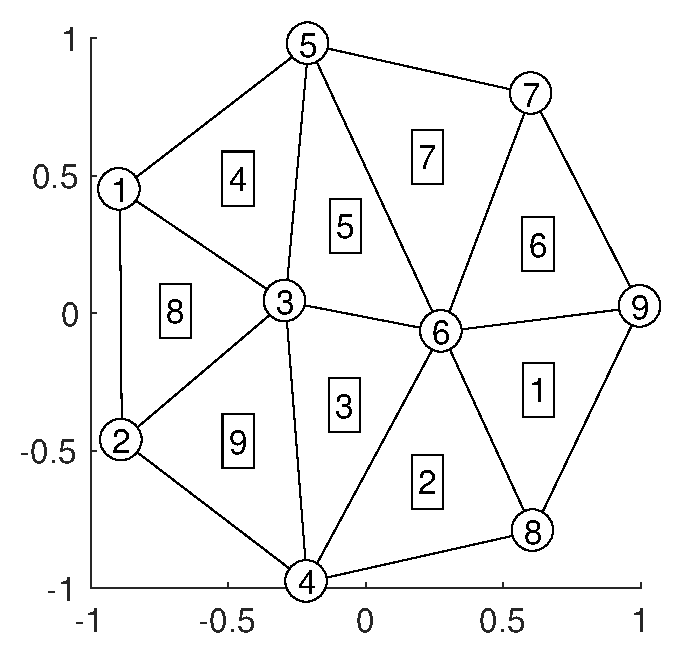
\includegraphics[width=0.4\textwidth]{mesh_p1}
  \caption{Example $p=1$ mesh.}
\end{figure}

\begin{itemize}
\item \texttt{coord}. $n_{\rm node} \times 2$ array of node coordinates. For a linear mesh ($p=1$), the array comprise the coordinates of all vertices.  For a quadratic mesh ($p=2$), the array comprise the coordinates of all vertices and mid-edge nodes.
\begin{verbatim}
>> mesh.coord

ans = 

   -0.8936    0.4489
   -0.8865   -0.4628
   -0.2916    0.0425
   -0.2129   -0.9771
   -0.2075    0.9782
    0.2770   -0.0676
    0.6038    0.7971
    0.6101   -0.7923
    0.9997    0.0233
\end{verbatim}
\item \texttt{tri}. $n_{\rm tri} \times 3$ (or $n_{\rm tri} \times 6$) array of element-to-node connectivity for $p=1$ (or $p=2$) mesh.  For each element, we assume that the vertex nodes (i.e. the first three nodes) are ordered in the counter-clockwise manner. For $p=2$, the mid-edge nodes (i.e. the last three nodes) must be ordered in a manner consistent with the respective vertex nodes.
\begin{verbatim}
>> mesh.tri

ans =

     9     6     8
     8     6     4
     4     6     3
     3     5     1
     6     5     3
     7     6     9
     7     5     6
     2     3     1
     4     3     2
\end{verbatim}
%\item \texttt{bgrp}. A cell array of the length equal to the number of boundary groups in the mesh.
\item \texttt{bgrp\{ibgrp\}}. $n_{\rm bgrp-edge} \times 4$ array containing boundary edge information, where $n_{\rm bgrp-edge}$ is the number of edges in the given boundary group.
  \begin{itemize}
  \item \texttt{bgrp\{ibgrp\}(i,[1,2])} is the two end nodes of the $i$-th boundary edge. We assume that the nodes are ordered such that the oriented edge traverses the element on the boundary in the counter-clockwise direction.
  \item \texttt{bgrp\{ibgrp\}(i,3)} is the element to which the $i$-th boundary edge belongs.
  \item \texttt{bgrp\{ibgrp\}(i,4)} is the local edge index for the element \texttt{bgrp\{ibgrp\}(i,3)} associated with the $i$-th boundary edge.
  \item The above definition implies that the two numbers returned by \texttt{bgrp\{ibgrp\}(i,[1,2])} should be equal to \texttt{mesh.tri(bgrp\{ibgrp\}(i,3), ref.e2v([1,2],bgrp\{ibgrp\}(i,4)))}.
  \item \emph{Note.} The first two columns of \texttt{bgrp\{ibgrp\}} are generated by the mesher function (e.g., \texttt{make\_square\_mesh}).  The third and fourth columns of \texttt{bgrp\{ibgrp\}} are computed and appended by the function \texttt{make\_bgrp}. In other words, \texttt{make\_bgrp} should append the \texttt{bgrp} structure, which originally only consists of the vertex information, with the associated boundary element information.
  \end{itemize}
\begin{verbatim}
>> mesh.bgrp{1}
   
ans =

     5     1     8     2
     8     9     4     1
     4     8     9     2
     9     7     2     2
     1     2     7     3
     2     4     6     2
     7     5     1     2
\end{verbatim}
\end{itemize}
We now provide a list functions.
\begin{itemize}
\item \texttt{make\_square\_mesh}, \texttt{make\_circle\_mesh}, etc. Create a mesh of the given shape.
\item \texttt{make\_bgrp}. Append the \texttt{.bgrp} field with the boundary element information. 
\item \texttt{add\_quadratic\_nodes}.  Add quadratic nodes to the mesh structure; i.e., converts $p=1$ mesh to $p=2$ mesh.  Both the \texttt{.coord} and \texttt{.tri} fields are modified by the function.
\item \texttt{nodes\_on\_boundary}.  Identify nodes on a given set of boundary groups.  The function is often used to impose Dirichlet boundary conditions.
\item \texttt{refine\_uniform}. Uniformly refine all elements.
\item \texttt{refine\_mesh\_nvb}. Refine marked elements.
\item \texttt{plot\_mesh}.  Visualize a mesh.
\item \texttt{plot\_field}. Visualize a field.
\end{itemize}

\section{The \texttt{ref} structure}
The \texttt{ref} structure contains information about the reference element.  We use the $p=1$ reference element with $p_{\rm quad} = 4$ quadrature rule to illustrate the construction.  The \texttt{ref} structure can be divided into multiple functional groups; we will describe each group separately.

The first set of fields define the 2d quadrature rule for the reference triangle.
\begin{figure}[!h]
  \centering
  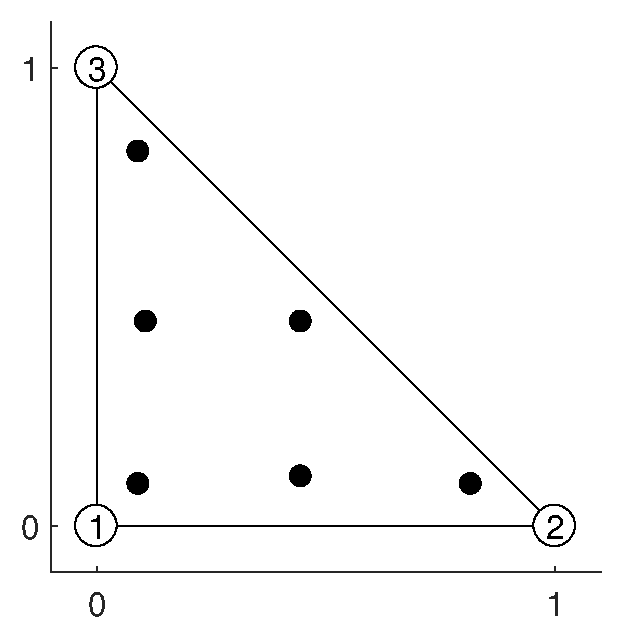
\includegraphics[width=0.4\textwidth]{ref_p1}
  \caption{Example $p=1$, $p_{\rm quad} = 4$ reference triangle element.  The interpolation nodes are numbered; the quadrature points are shown in dots ($\bullet$).}
\end{figure}
\begin{itemize}
\item \texttt{pquad}.  The degree of polynomials exactly integrated.
\begin{verbatim}
>> ref.pquad

ans =

     4
\end{verbatim}
\item \texttt{xq}. An $n_{\rm quad} \times 2$ array of the coordinates of the quadrature points, where $n_{\rm quad}$ is the number of quadrature points.
\begin{verbatim}
>> ref.xq

ans =

    0.0916    0.0916
    0.8168    0.0916
    0.0916    0.8168
    0.4459    0.4459
    0.1081    0.4459
    0.4459    0.1081
\end{verbatim}
\item \texttt{wq}. An $n_{\rm quad}$-vector of the quadrature weights.
\begin{verbatim}
>> ref.wq

ans =

    0.0550
    0.0550
    0.0550
    0.1117
    0.1117
    0.1117
\end{verbatim}
\end{itemize}
The next set of fields define the 2d shape functions on the reference triangle.
\begin{itemize}
\item \texttt{p}. The polynomial degree of the finite element.
\begin{verbatim}
>> ref.p

ans =

     1
\end{verbatim}
\item \texttt{xint}. An $n_{\rm shp} \times 2$ array of the coordinates of the interpolation nodes.  Here, $n_{\rm shp}$ is 3 and 6 for $p=1$ and $p=2$ element, respectively.
\begin{verbatim}
>> ref.xint

ans =

     0     0
     1     0
     0     1
\end{verbatim}
\item \texttt{shp}. An $n_{\rm quad} \times n_{\rm shp}$ array of the values of the shape functions evaluated at the quadrature points. \texttt{shp(i,j)} is the value of the $j$-th shape function at the $i$-th quadrature point.
\begin{verbatim}
>> ref.shp

ans =

    0.8168    0.0916    0.0916
    0.0916    0.8168    0.0916
    0.0916    0.0916    0.8168
    0.1081    0.4459    0.4459
    0.4459    0.1081    0.4459
    0.4459    0.4459    0.1081
\end{verbatim}
\item \texttt{shpx}. An $n_{\rm quad} \times n_{\rm shp} \times 2$ array of the gradients of the shape functions evaluated at the quadrature points. \texttt{shpx(i,j,k)} is the partial derivative of the $j$-th shape function in the $k$-th direction at the $i$-th quadrature point.
\begin{verbatim}
>> ref.shpx

ans(:,:,1) =

    -1     1     0
    -1     1     0
    -1     1     0
    -1     1     0
    -1     1     0
    -1     1     0


ans(:,:,2) =

    -1     0     1
    -1     0     1
    -1     0     1
    -1     0     1
    -1     0     1
    -1     0     1
\end{verbatim}
\end{itemize}
The next set of fields define the 1d quadrature rule on a unit line segment.  The 1d quadrature rule is used to integrate function on edges as required in, for example, integration of boundary quantities.
\begin{figure}[!h]
  \centering
  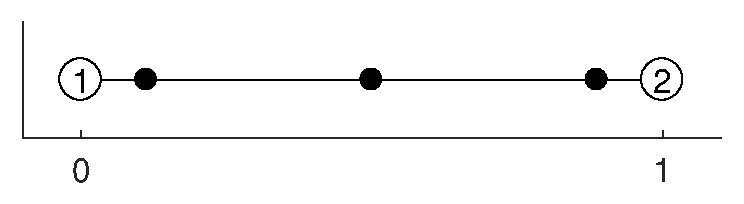
\includegraphics[width=0.4\textwidth]{ref_p1_1d}
  \caption{Example $p=1$, $p_{\rm quad} = 4$ reference edge element.  The interpolation nodes are numbered; the quadrature points are shown in dots ($\bullet$).}
\end{figure}
\begin{itemize}
\item \texttt{xqf}. An $n_{\rm quad-facet}$-vector of the coordinate of the 1d quadrature points, where $n_{\rm quad-facet}$ is the number of 1d quadrature points.
\begin{verbatim}
>> ref.xqf

ans =

    0.1127
    0.5000
    0.8873
\end{verbatim}
\item \texttt{wqf}. An $n_{\rm quad-facet}$-vector of 1d quadrature weights.
\begin{verbatim}
>> ref.wqf

ans =

    0.2778
    0.4444
    0.2778
\end{verbatim}
\end{itemize}
The next set of fields define the 1d shape functions on a unit line segment. 
\begin{itemize}
\item \texttt{shpf}. An $n_{\rm quad-facet} \times n_{\rm shp-facet}$ array of the values of the 1d shape functions evaluated at 1d quadrature points.
\begin{verbatim}
>> ref.shpf

ans =

    0.8873    0.1127
    0.5000    0.5000
    0.1127    0.8873
\end{verbatim}
\item \texttt{shpxf}. An $n_{\rm quad-facet} \times n_{\rm shp-facet}$ array of the derivative of the 1d shape functions evaluated at 1d quadrature points.
\begin{verbatim}
>> ref.shpxf

ans =

    -1     1
    -1     1
    -1     1
\end{verbatim}
\end{itemize}
The last field relates edge degrees of freedom to element degrees of freedom.  The field is used, for example, to identify boundary degrees of freedom.
\begin{itemize}
\item \texttt{f2n}. An $n_{\rm shp-facet} \times 3 \times 2$ array of edge-to-node connectivity information, where $n_{\rm shp-facet}$ is the number of interpolation nodes on an edge (i.e., $n_{\rm shp-facet} = 2$ and $3$ for $p=1$ and $2$, respectively). \texttt{f2n(i,j,1)} is the $i$-th interpolation node on the $j$-th edge when the edge is oriented in the natural direction (i.e., along the counter-clockwise orientation of the element). \texttt{f2n(i,j,2)} is the $i$-th interpolation node on the $j$-th edge when the edge is oriented in the reverse direction (i.e., along the clockwise orientation of the element).
\begin{verbatim}
>> ref.f2n

ans(:,:,1) =

     2     3     1
     3     1     2


ans(:,:,2) =

     3     1     2
     2     3     1
\end{verbatim}
\end{itemize}
We now provide a list of functions.
\begin{itemize}
\item \texttt{interp\_nodes\_\{tri,line\}}.  Returns Lagrange interpolation nodes.  Used to fill the \texttt{.xint} field of the \texttt{ref} structure.
\item \texttt{quad\_\{tri,line\}}.  Returns quadrature points and weights.  Used to fill the \texttt{.xq}, \texttt{.wq}, \texttt{.xqf}, and \texttt{.wqf} fields of the \texttt{ref} structure.
\item \texttt{monomial\_\{tri,line\}}.  Evaluates the shape function values and gradients associated with monomial basis.  Provides basis function from which the Lagrange shape functions are generated using \texttt{shape\_\{tri,line\}}; the function is rarely used by its own.
\item \texttt{shape\_\{tri,line\}}.  Evaluates the shape function values and gradients associated with Lagrange basis.  Used to fill the \texttt{.shp}, \texttt{.shpx}, \texttt{.shpf}, and \texttt{.shpxf} fields of the \texttt{ref} structure.
\item \texttt{make\_ref\_tri}.  A high-level function that fills in all the fields of the \texttt{ref} structure.
\end{itemize}
\end{document}

